\chapter{Evaluating City-Level Communities using Location Data}\label{chap4}

\setlength{\abovedisplayskip}{-10pt} \setlength{\abovedisplayshortskip}{-10pt}

\section{Introduction}
Chapter 3 proposed a method for identifying city-level communities and associated geo-influencers. The method works via: (i) automated Google search queries to get an initial set of city-level geo-influencers, (ii) the followers of these geo-influencers used for forming city-level communities, (iii) the follow connections from communities used for identifying additional geo-influencers. TF-IDF model, where the terms are influencers, generates a ranked list of local influencers for each city-level community. The method was tested using 64 cities of the USA. We have confirmed that there is an overlap between influencers that Google finds relevant and the ones identified via city-level communities built using a geocoder. In this chapter, we perform a more comprehensive evaluation that checks whether the central location from influencer's followers matches the city the influencer is associated with.

From related research, there are numerous approaches for generating a ranked list of location-aware influencers, but evaluation of these is typically performed by human annotators and is thus limited to small datasets. In this research, we fuse information from associations made by Google, links from the Twitter social network, and attributes from user profile information for automatically generating labels. This allows us to perform an evaluation that covers thousands of location-aware influencers across 763 cities within the USA.

The evaluation can be automated by checking if the city (associated via Google or TF-IDF ranking) of the geo-influencer matches the central location (via location features) from influencer's followers. The features proposed can be used to characterize known influencers in a type of repository that captures the geographic area they serve. 
%Maintaining such a repository would allow other researchers to leverage, as a starting point, those influencers within the geographic location of interest vs. having to perform time-intensive collection from scratch. 

Different ways for assigning a central location are illustrated on (i) Members of Congress for whom the label is the state that the congressman is known to serve and (ii) influencers associated with a city via Google search. The initial set of influencers extracted using Google are evaluated using (i) query (certain queries such as those that contain a city matching a person name are found to be more ambiguous), (ii) number of associated followers (a large enough sample of followers is needed to calculate the central location), and (iii) based on URL position (URLs Google recommends first may have higher confidence). 

Important findings of this research are that for cities in the USA: (i) 94.33\% of initial influencers returned by Google had their central location match the city being queried, (ii) city-level community that is based on the intersection of followers of multiple city-level geo-influencers is better aligned to the city, and (iii) a classifier for differentiating city-level geo-influencers in the USA vs. national and foreign influencers is possible without a geocoder dedicated to other languages. The approach described in this chapter should be applied to verify that the geo-influencers and the resulting city-level communities for the USA from chapter 3 are accurate.

\section{Related Research}
Location-Aware Influence Maximization (LAIM) aims to rank influencers based on the underlying geographic population [\ref{appendix:3.1}, \ref{appendix:3.2}]. %A few examples of city influencers include mayor, city's police, local news, local businesses, and local sports [\ref{appendix:3.3}, \ref{appendix:2.26}]. 
The content posted by these influencers can be analyzed for understanding preferences of the underlying population which can aid in personalized recommendations and targeted advertisement [\ref{appendix:3.5}]. The followers of influencers can be used for forming communities and understanding how they differ in overall depression [\ref{appendix:3.6}], crime [\ref{appendix:3.7}], happiness [\ref{appendix:3.8}], and other factors.

%Locations on Twitter come from user's profile, user coordinates recorded while posting a message, and location mentioned within message contents [\ref{appendix:1.1}]. %The residential address associated with a user typically comes from the self-reported textual profile location or aggregated from coordinates in user's messages. Messages with geo are limited to 1-3\% of the overall Twitter stream and may bias results towards a specific group such as wealthier individuals who travel more [\ref{appendix:1.12}]. Self-declared textual location is available for up to 45\% of users, but it needs to be accurately geocoded to latitude and longitude coordinates [\ref{appendix:3.11}]. Users without location information may be assigned to the median of their friends' locations [\ref{appendix:1.11}]. 
The current state of the art is to geocode available self-reported locations and infer the rest from friends' locations [\ref{appendix:3.13}]. Most researches choose to focus on US and English based tweets with user location aggregated at the city, county, and state levels [\ref{appendix:3.14}]. Language and time zone features are important for differentiating foreign country users [\ref{appendix:1.7}, \ref{appendix:3.15}]. 

Identifying location-aware influencers typically involves (i) collecting network, (ii) reducing the network to nodes matching the geographic location of interest, and (iii) extracting most important nodes via graph-based measures. %Due to Twitter's size, the complete social network link structure is not possible to extract. As a result a popular solution is to approximate the link structure from message traffic; if user A mentions user B form a link between A and B [\ref{appendix:2.26}]. 
Challenge of this approach is that it involves a large collection, sometimes involving billions of messages, that covers a geographical area much larger than is of interest. The method also misses passive users and overexposes itself to actively talking bots [\ref{appendix:3.17}]. %We chose an alternative approach, which iteratively refines the network via a targeted collection [\ref{appendix:3.3}].% that results in a larger and larger network.

The geographical area of interest is typically specified via a region bounded by some radius R [\ref{appendix:2.2}, \ref{appendix:2.26}]. The users whose home location falls within this radius are then part of the community. Once a community that is representative of the geographical area is established traditional measures such as closeness centrality, and more recently variations on the PageRank algorithm, are used to extract the most important influencers [\ref{appendix:2.1}]. %In [\ref{appendix:2.26}] a modified PageRank is used for identifying influencers within three regions, each with a radius of 100 km.
 
%Previous chapter illustrated an approach in which Google is used to identify an initial set of influencers associated with a city location, followers of influencers form communities, and communities used for identifying additional influencers via a modified TF-IDF measure [\ref{appendix:3.3}]. The benefit of the method is that (i) collection is orders of magnitude smaller than a comparable bottom-up approach, (ii) it incorporates direct follow links vs. approximations from message traffic, and (iii) it results in a superior list of influencers. With this approach some issues remain --- (i) the initial set of influencers identified via Google search are assumed to be correct and (ii) the evaluation data is limited to human annotation covering only a couple of cities with just dozens of accounts.

The outputs of competing influencer ranking algorithms can be compared via measures such as Spearman's correlation, Kendall's Tau, and Rank Biased Overlap (RBO) [\ref{appendix:3.21}]. The evaluation of whether an influencer is actually within the geographical area of interest is often neglected. Most often the influencers are assumed to be within the geographical area of interest based on their self-reported location or some other heuristic. 

Diffusion model is used for estimating how the influence propagates through the network using Independent Cascade, Linear Threshold, Triggering, or Time Aware models [\ref{appendix:3.1}]. Simulations helpful for understanding the overlapping effect between followers [\ref{appendix:3.22}]. Models help evaluate the best set of influencers to trigger a large cascade of further adoptions of a new behavior based on a contagion process [\ref{appendix:3.23}, \ref{appendix:3.24}]. These simulation models may contain mistakes if the influencer is not from the geographical area of interest. 

The evaluation of whether an influencer is actually within the geographical area of interest is often limited to manual human efforts. For example, ground truth may consist of influencers that are discovered by human annotators and the algorithm is evaluated based on the percent of ground truth influencers identified [\ref{appendix:2.26}, \ref{appendix:3.3}]. Such evaluations contain human bias and are limited to at most dozens of influencers across a handful of locations.

\section{Assign Central Location (ACL)}

This section describes the approach for automatically assigning a central location to each influencer. Our focus is on high confidence self-reported locations that contain both the city and state abbreviation [\ref{appendix:1.9}]. Let set $C$ represent 763 US cities as possible values for the central location\footnote{Cities are from US Census Bureau, are representative of all states plus DC, and have a population of over fifty thousand (some exceptions such as Burlington largest city in VT)} and $F(u)$ represent set of followers associated with influencer $u$. $D(F(u), c)$ gives the ratio of self-reported locations from followers of influencer $u$ that map to city $c$:

\begin{equation}
\label{eqn_DFu}
D(F(u), c) = \frac{
\text{followers  mapping  to  city  }c}{\sum_{k=1}^{763}\text{followers mapping to city } c_k}
\end{equation}

A lowercase city-state string represents each city $c$ (without whitespace or punctuation), example `newyorkny'. Each follower's self-reported location is turned to lowercase with punctuation and whitespace stripped out. The preprocessed location is utilized if it matches one of the cities in set $C$. Examples of self-reported locations that map to city `newyorkny': `NewYorkNY', `New York, NY :)', `New York,NY'. D(F($u$), $c$) values form a distribution over all cities. As an example top three values for influencer @ChicagoTribune correspond to: `chicagoil': 0.553, `washingtondc': 0.026, and `newyorkny': 0.019. The central city $c$ location for influencer $u$ is given by:

\begin{equation}
C1(u) = c^* \text{ where } D(F(u), c^*) = \max_{c \in C}\{D(F(u), c)\}
\end{equation}

\begin{eqnarray}
C2(u) & = & c^* \text{ where } D(F(u), c^*) \\ \nonumber
& = & \min_{c \in C}\{\sum_{k=1}^{763} \ V(c_k, c)*D(F(u), c_k)\}
\end{eqnarray}

\begin{equation}
C3(u) = c^* \text{ minimizes } V(c^*, {\sum_{k=1}^{763} \ L(c_k) * D(F(u), c_k)})
\end{equation}

\noindent where $V(c_1, c_2)$ is the Vincentry's distance [\ref{appendix:1.17}] between coordinates associated with city $c_1$ and $c_k$; $L(c_k)$ gives the latitude and longitude associated with city $c_k$.

$C1(u)$ gives the city $c$ that captures the largest ratio of influencer $u$'s followers. $C2(u)$ gives the city $c$ with the smallest average measure (distance between city and neighbor times frequency associated with neighbor) across all city neighbors. $C3(u)$ is the city $c$ whose coordinates are closest to the average latitude and longitude.

Let $L(u)$ specifies latitude, longitude coordinates at the center of the geographic area that the influencer $u$ is supposed to serve. In future sections, such a label can come from the city that Google associates with an influencer, state associated with a member of Congress, or a city using TF-IDF measure. The error distance (ED) is the Vincenty's distance from the coordinates in label $L(u)$ to computed central location $C(u)$ (where $C(u)$ can be $C1(u)$, $C2(u)$, or $C3(u)$):

\begin{equation}
\label{eqn_ED}
ED(u) = distance(L(u), C(u))
\end{equation}

Across a set of influencers $U$ we can calculate corpus level metrics (1) Mean ED, (2) Median ED, and (3) ED@X; percent of influencers confirmed by followers within X miles of central location; precisely defined below. Median ED is usually less sensitive than Mean ED for wildly inaccurate predictions. For ED@X, X = 0 corresponds to exact city matches whereas X = 100 considers city matches within 100 miles\footnote{X=100 is a popular distance for categorizing mismatch between the user's self-reported location and location inferred from messages [\ref{appendix:1.1}]}. 

\begin{equation}
MeanED = \frac{1}{|U|}\sum_{u \in U}\ ED(u)
\end{equation}

\begin{equation}
MedianED = \underset{u \in U}{\mathrm{median}} \{ED(u)\}
\end{equation}

\begin{equation}
ED@X = \frac{|\{u \in U|ED(u)\leq X\}|}{|U|}
\end{equation}

\section{Verification using Members of Congress}

Influencers consisting of 463 members of Congress were used to test the ACL process. At most 500K followers were sampled per influencer. In the dataset so obtained our goal was to check whether the central location computed from Congressman's followers matches the home state that the Congressman is known to serve. For example, if a Congressman is known to represent the state of Nebraska will his followers be concentrated around the same state. The central location for each influencer comes from the ACL process using (i) city distribution and assigning state from the associated city centroid or (ii) directly computing state centroid from state distribution (by aggregating 763 cities into 50 states + DC). Table \ref{table_4_1} shows performance using ED@0 and Mean ED.

\begin{table}
\small
\caption[Percent of Congressmen whose followers confirm home state]{Percent of Congressmen whose followers confirm home state. For each central location calculation (ED@0, Mean ED) are shown.}
\label{table_4_1}
\begin{center}
\begin{tabular}{|c|c|c|c|}
\hline
\bfseries Distribution & \bfseries C1 & \bfseries C2 & \bfseries C3\\
\hline
city&20.3\%, 789.82&\bfseries 27.65\%, 483.02&4.54\%, 596.51\\
\hline
state&\bfseries 53.35\%, 389.38&33.69\%, 452.35&6.05\%, 595.74\\
\hline
city (DC off)&\bfseries 93.3\%, 72.43&61.99\%, 227.72&9.72\%, 563.32\\
\hline
state (DC off)&\bfseries 90.06\%, 188.43&66.31\%, 227.5&6.91\%, 558.23\\
\hline
\end{tabular}
\end{center}
\end{table}

The first two rows show performance that is penalized due to the majority of members being associated with DC. For example, the C1 column in the first row had 368 out of 463 members (79.5\%) associated with DC, but the other 93 out of 95 members (97.9\%) were accurately associated with the Congressman's home state. Similarly, C1 column in the second row had 203 out of 463 members (43.3\%) associated with DC with the other 246 out of 260 members (94.6\%) being accurate. DC is a reasonable point of influence for members of Congress, but we experimented with whether the home state can be retrieved if DC is not an option.

The last two rows show performance if Washington DC is removed from the frequency distribution. The best results were using C1 with city distribution where the home state was matched for 433 out of 463 members. In-depth analysis of 30 Congressmen that did not match their home state showed that either they had a large national following (such as Speaker Ryan, Senator Sanders, and Senator Warren) or were mixed with a neighboring state (for example @senatormenendez, @billpascrell, @frankpallone, @repchrissmith, @replobiondo, @replancenj7, @usreprodney, @reptommacarthur, and @repbonnie represent the state of NJ but most of the followers associated with the state of NY).

This section confirms our hypothesis that location-aware influencers can be identified by the location that captures the biggest percent of the influencer's followers. We observed that C1 performs the best using city distribution. It is important to consider C2 since it compares the city to every other city within the distribution. When C2 matches C1, it means that locations outside of C1 are either clustered around it or do not carry enough weight to shift it. For this dataset, there was a significant discrepancy between C1 and C2 because the Congressman's influence was often divided between DC and Congressman's home state. C3's poor performance highlights that a simple mean of coordinates is not well suited for this problem (C3 was tested on other datasets with similarly poor results and as a result is not mentioned in future sections). 

\section{Features}


Geocoded location, time zone, and language are often described as the most important features for differentiating between users [\ref{appendix:1.7}, \ref{appendix:3.15}]. Geocoded location and language were utilized (timezone not used as it became a private field in 2018). In all 20 features were proposed as shown in Table \ref{table_4_2}. 

Features have discriminatory characteristics for identifying city vs. global influencers, as evident from values associated with @ChicagoTribune (a city influencer) and @CNN (a global influencer) which will be applied in a classifier in Section 4.9. As described in section 4.3 the influencer's followers' self-reported locations were used for generating a frequency distribution over 763 cities. 
This distribution was used for calculating C1 and C2 which serve as F1 and F2 features. 

\begin{table}
\small
\caption{Proposed Features}
\label{table_4_2}
\begin{center}
\tabcolsep=0.1cm
\begin{tabular}{|c|c|c|}
\hline
\bfseries F & \bfseries Description & \bfseries CNN vs ChicagoTribune\\
\hline
F1,&Centroid based on most frequent city (C1), &(losangelesca, stlouismo)\\
F2&Centroid based on mean coordinate (C2),& vs. (chicagoil, chicagoil)\\
\hline
F3&Vincenty's distance between (C1, C2)&1589.4 mi vs. 0 mi\\
\hline
F4&Number of followers that the influencer has&41275970 vs. 1069351\\
\hline
F5&Number of followers collected&991992 vs. 1060039\\
\hline
F6&Followers from F5 with non-empty location&451897 vs. 414695\\
\hline
F7&Followers from F6 mapping to one of 763 cities&43717 vs. 144580\\
\hline
F8&Percent of followers with non-empty &9.7\% vs. 34.9\%\\
&locations used in distribution: F7/F6&\\
\hline
F9, &C1 and C2 radius: average Vincenty &1440.8, 895.6 mi vs. \\
F10&distance from centroid to all other city&314.3, 314.3 mi\\
&sensors within distribution&\\
\hline
F11, &Ratio of followers captured by city &5.8\%, 0.6\% vs. \\
F12&centroid C1 and C2, respectively.&55.3\%, 55.3\%\\
\hline
F13, &Follower sample ratio mapping to centroid:&0.56\%, 0.058\% vs. \\
F14&F8*F11, F8*F12 for C1, C2.&19.3\%, 19.3\%\\
\hline
F15, &Ratio of followers captured by city/Ratio &1.8, 2.5 vs. \\
F16&of population captured by city where city is&25.5, 25.5\\
&associated with C1 and C2, respectively&\\
\hline
F17&P-value from Kolmogorov-Smirnov test &0.562 vs. 0.789\\
\hline
F18&ratio captured by English language&81.6\% vs. 90.7\%\\
\hline
F19&most frequent non-English language&Spanish vs. Spanish\\
\hline
F20&ratio captured by F19&4.5\% vs. 3.5\%\\
\hline
\end{tabular}
\end{center}
\end{table}


City distribution, user profile information, and centroids used for calculating features F3-F14 as shown in the table. Distribution of the population was obtained by dividing the population of a city by the population across all 763 cities (using US Census populations). 763 city distribution and population distribution used for calculating features F15-F17. Finally, the preferred follower's profile language used to generate a language distribution over all influencer's followers for features F18-F20. 

\section{Approach}

\begin{figure}[htbp]
\centerline{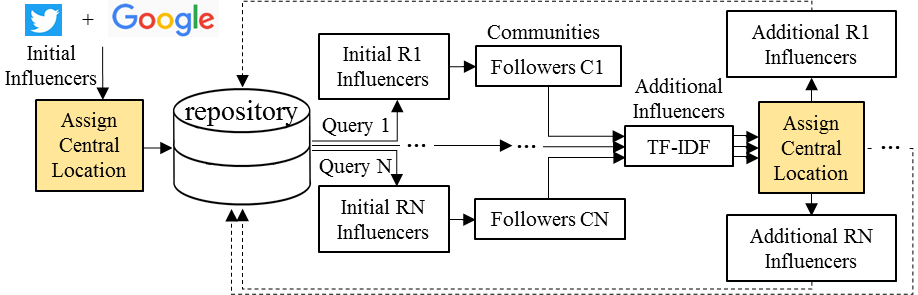
\includegraphics[width=5.4in]{fig1.png}}
\caption{Establishing and continuously updating a repository of influencers.}
\label{fig_ch4_1}
\end{figure}

Our proposed solution for building and continuously updating a repository of geo-influencers is illustrated in Fig.  \ref{fig_ch4_1}. The process extends the approach from previous chapter via the Repository and ACL process (highlighted in yellow). The required inputs are the geographic regions of interest over which influencers will be collected. A city-level location is the smallest geographic area considered since this is a popular choice among Twitter users [\ref{appendix:3.11}]. 

Larger geographical areas can be formed from cities along recognized political boundaries; cities make up fifty states, states combined into nine divisions, and divisions combined into four regions of US. Examples of system input would then be Syracuse NY vs. Buffalo NY (city), NY vs. PA (state), Mountain vs. Pacific (divisions), and Northeast vs. Midwest (regions). This section describes experiments with city and state as regions. R1 to RN geographic regions with N\textgreater1 are expected so as to be able to apply the TF-IDF measure. The main processes from Fig. \ref{fig_ch4_1} are described below:

\begin{itemize}
\item Initial Influencers: Twitter influencers from automatic Google searches related to cities making up the geographic regions.

\item Assign Central Location (ACL): the central location assigned to each influencer based on the distribution exhibited by the influencer's followers, see section 4.3. 

\item Repository: stores centroids from ACL and additional features such as percent of followers captured by the centroid, average radius, and others, see section 4.5. Repository also stores whether influencer is local or global to country of interest using classifier from Section 4.9.

\item Query: repository queried for local influencers whose C1 centroid matches the geographic region of interest. Each query can contain additional inputs such as the minimum percent of followers associated with the region. 

\item Communities and Additional Influencers: Followers of influencers from regions R1 to RN form communities C1 to CN, respectively. Influencers that these communities follow are ranked via TF-IDF. Top influencers from TF-IDF go through the ACL process and stored in the repository for future reference. 
\end{itemize}

Additional influencers refine communities associated with each geographic region and the whole process shown in Fig. \ref{fig_ch4_1} can repeat. %How the ACL process can be used to improve initial influencers coming from Google and additional influencers stemming from TF-IDF is described next. The classifier for filtering out global users described in section 4.9.

\section{Analyzing Geo-Influencers Recommended by Google}

%Initial influencers stem from automatic Google searches. %For each query, the URLs of interest are those that have the domain: `twitter.com/'. If after domain there are no backslashes, the text is used as screenname with `?lang=en' stripped out. 
%As an example, Table 4.3 shows screennames extracted from top five URLs associated with query `Syracuse, NY Twitter'. %Each extracted Twitter screenname is verified to exist on Twitter. 


\begin{table}
\small
\caption{Top Ranked URLs via Google Search for `Syracuse, NY Twitter'}
\label{table_4_3}
\begin{center}
\begin{tabular}{|c|c|c|}
\hline
\bfseries Hit & \bfseries URL & \bfseries Influencer\\
\hline
0&https://twitter.com/syracuse1848?lang=en&syracuse1848\\
\hline
1&https://twitter.com/syracuseu?lang=en&syracuseu\\
\hline
2&https://twitter.com/hashtag/syracuse?lang=en&\\
\hline
3&https://twitter.com/syracuseunews?lang=en&syracuseunews\\
\hline
4&https://twitter.com/syracusedotcom&syracusedotcom\\
\hline
\end{tabular}
\end{center}
\end{table}

Initial influencers stem from automatic Google searches. As an example, Table \ref{table_4_3} shows screennames extracted from top five URLs associated with query `Syracuse, NY Twitter'. The order of returned URLs is recorded. It was expected that the influencers extracted from first web hits will have a higher correlation to the city queried. Fig. \ref{fig_ch4_2} shows the number of influencers extracted per URL using the top 100 URLs. Queries performed across 763 city state pairs where the number of influencers per city ranged from 1 to 33. Over these cities, there were a total of 14092 influencers, 13050 remained after removing influencers associated with multiple city queries or whose followers had no location information.

\begin{figure}[htbp]
\centerline{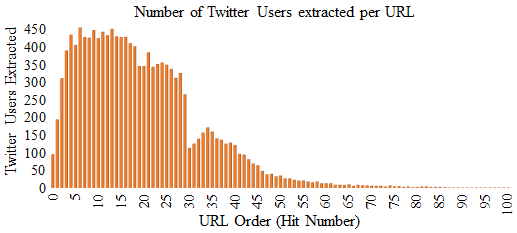
\includegraphics[width=5in]{fig2.png}}
\caption{Number of Twitter Users extracted via Google using top 100 URLs}
\label{fig_ch4_2}
\end{figure}

Next, a maximum of one million followers was collected for each influencer. Influencer's followers' self-reported locations were used to generate a distribution and compute centroids as described in Section 4.3. Error distance (\ref{eqn_ED}) computed between coordinates associated with the city queried vs. the central location coordinates from influencer's followers. Across all influencers ED@0 was 73.58\% for C1 and 70.11\% for C2. The subsections below examine the performance based on the query type, the follower sample size, and URL order.

\subsection{Performance based on Query Type}

Mean ED, Median ED, ED@0, and ED@100 were calculated across the influencers associated with each city query. Table \ref{table_4_4} shows the average and standard deviation for C1 and C2 centroids across queries. It is time consuming to analyze thousands of influencers via manual validation, but with the error measures proposed, we can quickly focus in on those queries that are problematic for Google. 

\begin{table}
\small
\caption{Average Performance across Google's Queries}
\label{table_4_4}
\begin{center}
\begin{tabular}{|c|c|c|}
\hline
\bfseries Error Measure & \bfseries C1 & \bfseries C2\\
\hline
Mean ED&53.89 +/- 164.63&63.17 +/- 150.64\\
\hline
Median ED&19.74 +/- 160.63&16.81 +/- 133.23\\
\hline
ED@0&0.69 +/- 0.32&0.66 +/- 0.29\\
\hline
ED@100&0.95 +/- 0.12&0.92 +/- 0.13\\
\hline
\end{tabular}
\end{center}
\end{table}

Out of 763 queries, only fourteen queries had ED@100 under 50\%. Thus most of Google's city-influencer associations are confirmed by the central location from influencer's followers. The problematic queries are described below.

One type of mistake stems from matching influencer not on location but based on screenname, description, or user specified name. Example of cities with human names are Lawrence MA (out of 8 influencers, city from query matched 0\% of self-reported locations, but matched 100\% of names example Jennifer Lawrence) and Anderson IN (out of 27 influencers, city from query matched 7\% of self-reported locations, but matched 96\% of names example Anderson Cooper). Contrast this to Trenton NJ where out of 27 influencers, the city from query matched 78\% of self-reported locations but matched only 52\% of names. 

Another mistake is related to state abbreviations that can be interpreted as a preposition (`OR' and `IN'). Nine out of fourteen queries faced this challenge: Gary IN, Albany OR, Anderson IN, Lafayette IN, Salem OR, Springfield OR, Gresham OR, Hillsboro OR, and Medford OR. Spelling out the state name might help these queries, i.e. Oregon instead of OR. The state name should not be spelled out for all queries because Google has more data for more common queries. For example, in the previous chapter we saw that typing out `New York, New York' causes Google's search to favor results associated with a casino in Nevada of the same name. This is again observed in that for `New York, New York Twitter' @NYNYVegas was the second URL recommended, i.e., spelling out the state name might also bring unintended results.

Finally, there were city names that are not unique to a single state. For example, there are 34 states with Springfield cities. Table \ref{table_4_5} shows specific instances where the wrong influencer was matched to query Albany OR and associated true location.

\begin{table}
\small
\caption{Google Mistakes for Query `Albany, OR Twitter'}
\label{table_4_5}
\begin{center}
\tabcolsep=0.15cm
\begin{tabular}{|c|c|}
\hline
\bfseries Albany OR Associated Influencers & \bfseries True Loc\\
\hline
albanyairport, albanysym, dutchmenpgcbl, reinventalbany &Albany, NY\\
\hline
naschoolupdates, newalbanyohio&Albany, OH\\
\hline
ahshuskies, ahuskiebaseball&Albany, MN\\
\hline
albanyassociate, albanymusicuk, thealbanyse8&UK\\
\hline
\end{tabular}
\end{center}
\end{table}

\subsection{Performance based on the follower sample size}

As described in Section 4.3 the central location is computed from influencer's followers' self-reported location distribution. For a small number of followers, there might not be enough locations to generate a proper distribution and associated centroid.

Fig. \ref{fig_ch4_3} (top) shows ED@0 error for C1 and C2 centroid as influencers with an increasing number of followers are considered. The figure illustrates that at least 500 followers are needed to get a large enough sample for computing the centroid. Because most of the influencers are associated with city level locations they, in general, cater to a smaller audience: 20\% had 500 and 54\% had 2000 followers or less.

\subsection{Performance based on Query Result Order}

First web hits have a much higher click-through rate. As a result, it was tested whether the influencers that are in the top results (low hit number) would have a higher accuracy in being associated with city query. 

Fig. \ref{fig_ch4_3} (bottom) shows ED@0 error for C1 and C2 on influencers grouped by hit number 0 to 29. Top 30 web hits were chosen because each had a good sample of Twitter influencers ranging from 387 to 490. The figure shows that the results remain about the same for influencers that appear in top vs. later web results. A possible explanation is that for ambiguous queries Google will have poor results across the board. 

\begin{figure*}[htp]
\centering
   \subfloat[Influencers grouped by number of followers]{\label{fig_ch4_3a}
      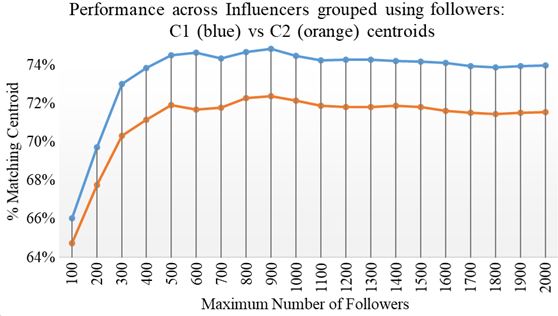
\includegraphics[width=.65\textwidth]{fig3}}
\\
   %\hspace*{\fill}   % maximize separation between the subfigures
   \subfloat[Influencers grouped by URL position from Google search]{\label{fig_ch4_3b}
      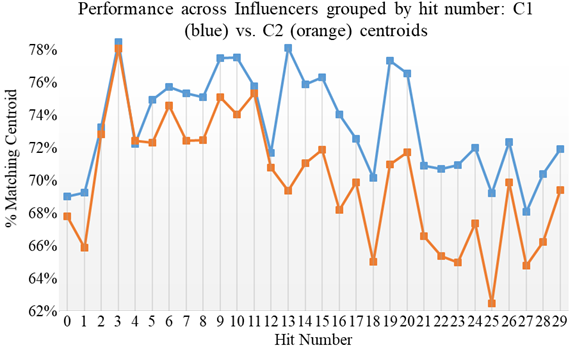
\includegraphics[width=.65\textwidth]{fig4}}
   \caption[Performance based on Follower sample size and Query order]{\textbf{Top} -- Performance based on Follower sample size. 500 or more followers provide a good sample for centroid calculation. \textbf{Bottom} -- Results from top 30 URLs illustrate that influencers in top web search results have similar performance as influencers in later web results.} \label{fig_ch4_3}
\end{figure*}

\iffalse
\begin{figure}[htbp]
\centerline{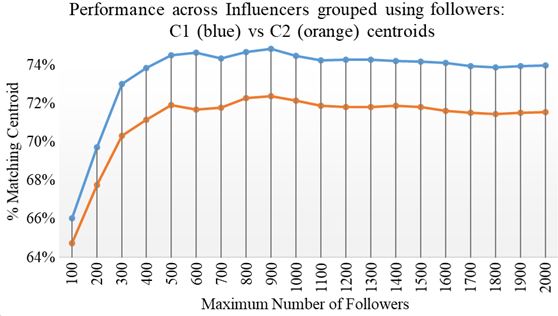
\includegraphics[width=4in]{fig3.png}}
\caption[Performance based on Follower sample size and Query order]{Performance based on Follower sample size. 500 or more followers provide a good sample for centroid calculation.}
\label{fig_ch4_3}
\end{figure}

\begin{figure}[htbp]
\centerline{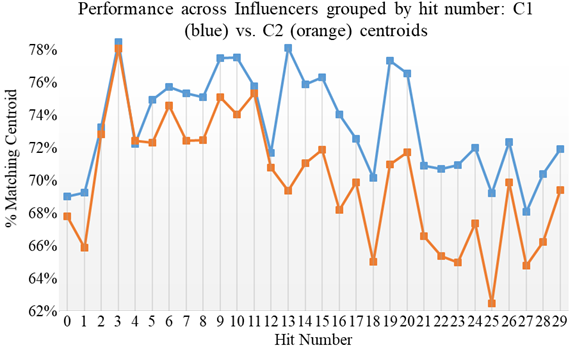
\includegraphics[width=4in]{fig4.png}}
\caption[Results based on order of top URLs]{Results from top 30 URLs illustrate that influencers in top web search results have similar performance as influencers in later web results.}
\label{fig_ch4_4}
\end{figure}
\fi

\iffalse
\section{Improving Influencers from TF-IDF}

As was shown in Fig. \ref{fig_ch4_1} the initial influencers from Google are used to form communities and discover additional influencers via TF-IDF. The dataset for this task consists of the top one-hundred influencers across 80 cities where each city was at least thirty miles away from the others and each city had at least ten Google associated influencers. Across these cities 94.33\% of initial influencers from Google had their C1 centroid match the city being queried. 7245 out of 8000 influencers remain after removing those overlapping multiple cities. A maximum of one million followers was collected for each influencer. This section examines performance based on the city and explores optimal city communities.

\subsection{Performance based on City Location}

Table \ref{table_4_6} shows cities with the least number of influencers matching the associated C1 centroid (ordered by ED@100). Salem OR and Medford OR contribute the most errors with much lower error rates for other cities. These results are unsurprising since these correspond to ambiguous Google queries discussed in Section 4.7 (errors in initial influencers from Google lead to communities that are not representative of the underlying geographical area). 

\begin{table}
\small
\caption{Ten worst performing cities using C1 centroid}
\label{table_4_6}
\begin{center}
\begin{tabular}{|c|c|c|c|c|}
\hline
\bfseries City Query & \bfseries MeanED & \bfseries MedianED & \bfseries ED@0 & \bfseries ED@100\\
\hline
Salem OR&997.34&793.38&0&0\\
\hline
Medford OR&679.98&0&0.59&0.59\\
\hline
Shreveport LA&140.03&0&0.66&0.67\\
\hline
Albany GA&102.42&0&0.76&0.77\\
\hline
Duluth MN&41.3&0&0.8&0.8\\
\hline
Dothan AL&70.51&0&0.67&0.83\\
\hline
Bismarck ND&63.5&0&0.84&0.84\\
\hline
Albany NY&116.27&0&0.85&0.86\\
\hline
Augusta GA&151.28&0&0.8&0.86\\
\hline
Salinas CA&152.98&0&0.69&0.87\\
\hline
\end{tabular}
\end{center}
\end{table}

Conversely, the top city communities had 100\% of influencers match C1 centroid (ED@0 = 0): Knoxville TN, Buffalo NY, Wichita KS, Springfield MO, Louisville KY, Syracuse NY, Boston MA, Charlotte NC, Pittsburgh PA, and Denver CO. For each of these cities, for each influencer, the city associated by Google matched the C1 centroid from influencer's followers. This again illustrates that the city communities need to be established using influencers that are confirmed by the ACL process.
\fi

\subsection{Forming Optimal Communities}

The higher the concentration of followers associated with a geographic city the better they are for establishing a city community. As an example, Table \ref{table_4_7} (top) shows five influencers recommended by Google for Syracuse, NY (each confirmed by their respective C1 centroid). Out of these @syracusedotcom has the highest concentration of followers associated with the city (70.1\%) and is thus the best for establishing the associated city community. Table \ref{table_4_7} (bottom) shows the percent of followers from Syracuse NY that follow a pair of influencers. Despite @cuse{\_}mbb having only 21.5\% of its followers from Syracuse, the table shows it can be used to improve percentages associated with followers extracted from other influencers. In this way, if a researcher wanted to focus on users from Syracuse that are interested in basketball and news, then followers of @cuse{\_}mbb and @syracusedotcom could be chosen to establish the city community with 73\% of followers mapping to Syracuse. 

\begin{table}
\small
\caption{Percent Followers mapping to City for Single vs. Pair of Geo-Influencers}
\label{table_4_7}
\begin{center}
\begin{tabular}{|c|c|c|c|c|c|}
\multicolumn{3}{c}{\bfseries Percent Followers of a single Geo-Influencers mapping to City}\\
\hline
\bfseries Influencer & \bfseries Number Followers & \bfseries \%C1\\
\hline
syracusedotcom&87334&70.13\\
\hline
sucampus&10238&53.23\\
\hline
gosyracuseu&2495&45.65\\
\hline
cuse&138595&41.63\\
\hline
cuse{\_}mbb&261805&21.49\\
\hline
\multicolumn{3}{c}{}\\
\multicolumn{3}{c}{\bfseries Mutual Followers of Two Geo-Influencers better aligned to city}\\
\hline
\bfseries Influencer Pair & \bfseries Mutual Followers & \bfseries \%C1\\
\hline
syracusedotcom + @cuse{\_}mbb&2784&73\\
\hline
sucampus + @cuse{\_}mbb&415&55\\
\hline
gosyracuseu + @cuse{\_}mbb&396&67.5\\
\hline
cuse + @cuse{\_}mbb&3250&48.7\\
\hline
\end{tabular}
\end{center}
\end{table}

A user that follows two geo-influencers has a higher chance of being from the city than the one that follows a single geo-influencer. We analyzed the percent gain over all possible pairs of influencers, where both influencers were associated by Google with the same city and confirmed by C1 centroid from the ACL process. There were 15951 pairs that produced 500 or more mutual followers across 492 cities. On average the pair had an 11.1\% gain over a single influencer. 3275 pairs had $90-98$\% percent of followers matching city of interest across 137 cities. Focusing on these pairs would lead to better city communities. It is not recommended to use three or more influencers because the overlap in followers may be too small.% (for example @cuse{\_}mbb and @syracusedotcom both have over 87K followers, but only 2.7K overlap).

\section{Classifier for City-Level Geo-Influencers}

In this section, we generate a classifier for differentiating US city-level geo-influencers vs. influencers that are from foreign countries or have more global influence. Our approach illustrates that it is possible to differentiate the two types by only geocoding the locations associated with the USA. 

Our dataset contained a total of 8740 influencers: 350 global influencers vs. 8390 US city geo-influencers. 8390 geo-influencers are obtained from Google and TF-IDF ranking. The city that the geo-influencer is associated with is verified by C1 centroid from the ACL process, the associated city name is also within the influencer's self-reported location, and each influencer had at least 500 followers (to ensure a large enough sample size as discussed in Section 4.7.2). 350 global influencers obtained via manual Twitter searches: 250 influencers are popular worldwide such as webmd, spacex, twittersports; 100 influencers came from foreign countries such as (screenname: country): ttcnotices: Canada, dailysabah: Turkey, vesti{\_}news: Russia, live{\_}hindustan: India, greateranglia: UK, and others.

Numeric features F3-F18 from Table \ref{table_4_2} were normalized to between 0 and 1 range. Nearest Neighbor (k=20), Gaussian Naïve Bayes, Decision Tree, Random Forest, and Support Vector Machines (SVM) with a linear and radial kernel were tried as classifiers with 3 fold cross validation\footnote{Scikit-Learn package utilized for implementation: https://scikit-learn.org/}. Unbalanced classes were handled by providing weights to SVM and random forest classifiers; global influencers were weighted 0.999 vs. 0.001 for city influencers (i.e. an incorrectly classified global influencer penalized classifier 1000 to 1 to ensure that all global influencers are accurately classified). We also tried to balance out the dataset by random over-sampling of the minority class. SVM and Nearest Neighbor were the only classifiers which classified all global influencers accurately. Fig. \ref{fig_ch4_5} shows average accuracy for these classifiers using an increasing number of features (drop in accuracy is due to the USA geo-influencers being classified as global/foreign) . Features ranked through Recursive Feature Elimination (RFE) with linear SVM.

\begin{figure}[htbp]
\centerline{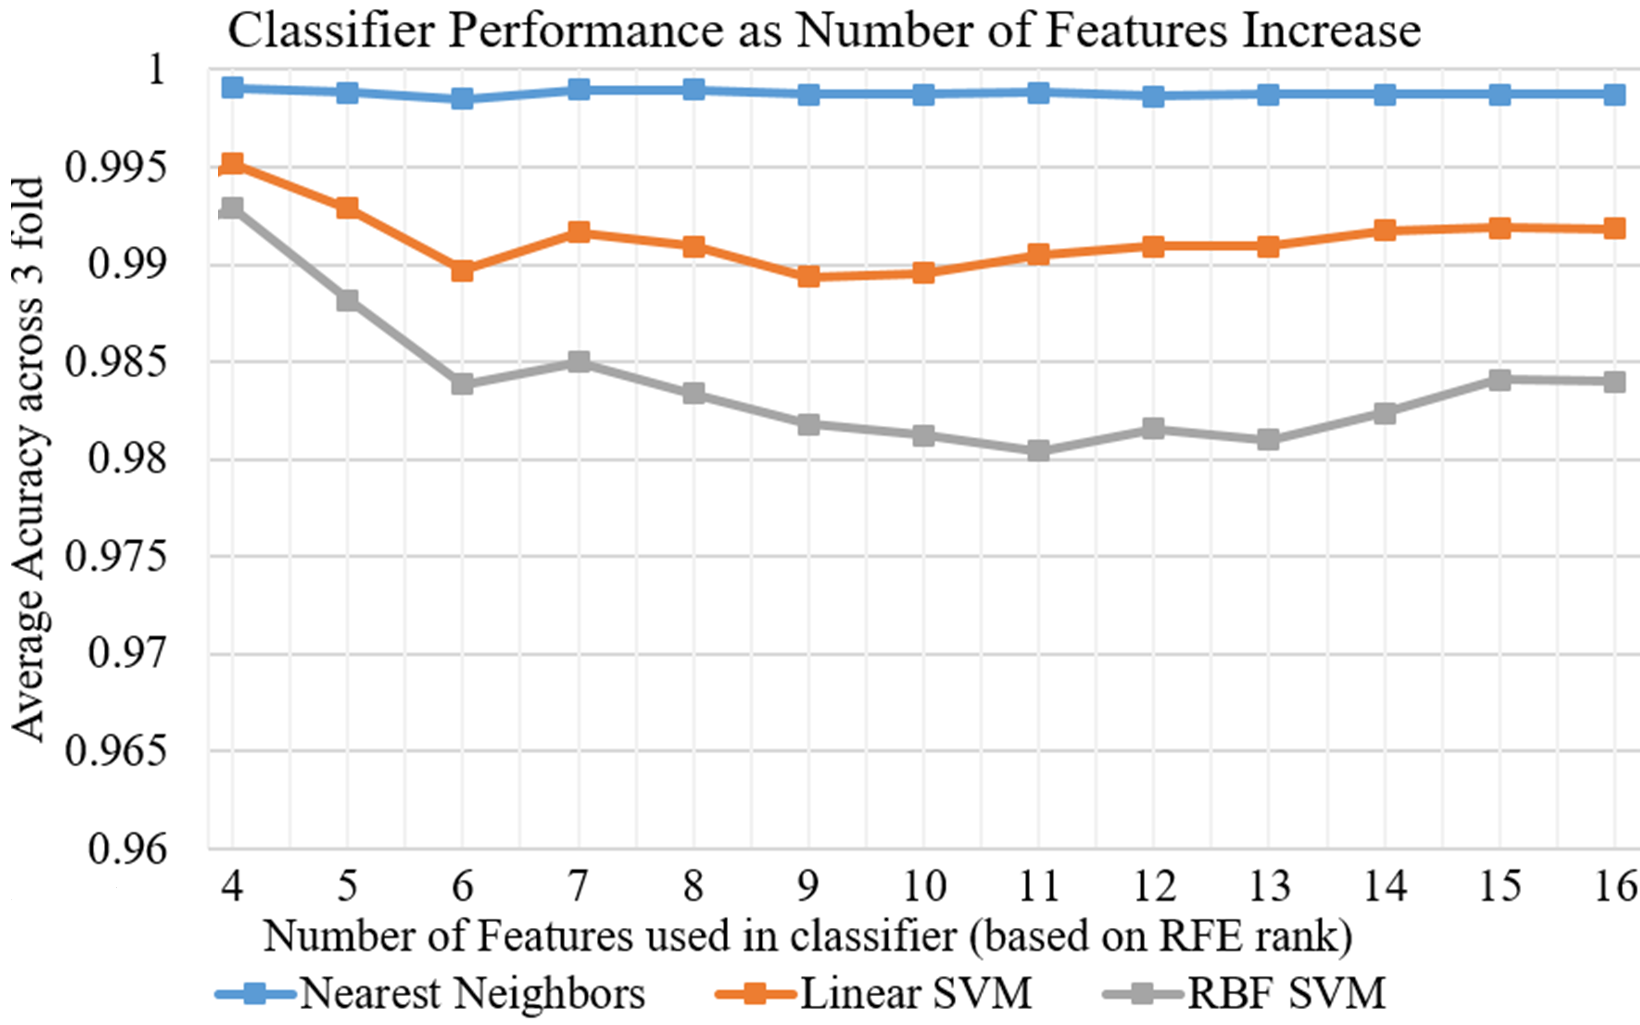
\includegraphics[width=5in]{fig5.png}}
\caption[USA vs. Foreign Country Classifier]{USA vs. Foreign Country classifier. Overall performance across three classifier peaks using top four ranked features.}
\label{fig_ch4_5}
\end{figure}

All three classifiers have peak performance when using the top four ranked features: F8 (percent followers mapping to US distribution), F13 (ratio of followers from sample mapping to C1 centroid), F7 (number of followers to US distribution), and F3 (distance between C1 and C2). Classifier performance using these four features illustrates that it is possible to differentiate US city vs. global influencers without having to geocode locations outside of the USA.

The results are intuitive in that influencers associated with a city $c$ in a country $x$ should (i) have a higher overall concentration of followers going to this country $x$ (necessary for filtering out influencers associated with foreign countries) and (ii) should exhibit an above average concentration of followers associated with the specific city $c$ (necessary for filtering out global influencers that may have a high concentration of followers in country x but whose influence spreads over many cities).

These are important results to consider because geocoding locations all around the world is difficult. For a specific country of interest, our recommendation is to focus on well-known cities within this country for forming a frequency distribution as was described in section 4.3. City influencers can then be extracted using a classifier and by focusing on those influencers verified by the C1 centroid. As the repository continues to grow in size the classifiers are expected to continue improving.

\section{Conclusions}
Our research proposed an automated evaluation for a targeted collection of influencers and corresponding city-level communities. The approach, described in this chapter, should be applied to verify that the geo-influencers and the resulting city-level communities for the USA from chapter 3 are accurate. 

The evaluation showed that Google does occasionally make mistakes for queries involving ambiguous city names (those that appear along with multiple states or that match popular human concepts). Our evaluation process allowed us to quickly identify these errors without having to review thousands of influencers manually. Queries with fewer than 50\% of influencers within 100 miles of the expected centroid (ED@100) were manually verified to be challenging for Google. The performance was about the same for influencers in top vs. later web results, i.e. web hit number does not play a significant role in how well influencer is associated with city query. Finally, it was shown that at least 500 followers are needed to have a large enough sample from which to compute the central location.

The method allowed to automate an evaluation covering thousands of influencers. Larger geographical areas were specified by aggregating multiple cities for a state-level evaluation. It was also illustrated how multiple influencers with a geographically local audience could be used to form city communities better aligned to the location of interest. Finally, a classifier was proposed for differentiating the USA vs. global and non-USA influencers; this classifier is possible without a geocoder dedicated to other languages. 

The methods described here are useful for generating and maintaining a repository of city-level influencers for the USA or other English-speaking countries (this is because the evaluation is still reliant on a gecoder that can process English-based locations). In the next chapter, we describe an approach that works worldwide by categorizing influencers using time-based features.

\iffalse
\subsection{Summary}

This section showed that Google does occasionally make mistakes for queries involving ambiguous city names (those that appear along with multiple states or that match popular human concepts). Our evaluation process allowed us to quickly identify these errors without having to review thousands of influencers manually. Queries with fewer than 50\% of influencers within 100 miles of the expected centroid (ED@100) were manually verified to be challenging for Google. The performance was about the same for influencers in top vs. later web results, i.e. web hit number does not play a significant role in how well influencer is associated with city query. Finally, it was shown that at least 500 followers are needed to have a large enough sample from which to compute the central location.
 
In general, if the query is unambiguous Google will do an excellent job in associating location-aware influencers with the city level location they serve, but Google cannot be always assumed correct. We improve the approach from reference [\ref{appendix:3.3}] by removing each influencer $u$ whose associated location is not confirmed by C1($u$) (2).
\fi